\chapter{PRISM}
\label{chap:prism}

\section{Introduction}
The complex spatiotemporal regulation of gene expression is a critical component in vertebrate development, evolution, and
disease~\citep{Levine2010, Visel2009}.  Understanding this regulation involves unraveling the cis-regulatory architecture,
namely the biological roles of transcription factors, their target genes in different biological contexts, and the regulatory
elements such as promoters and enhancers through which they exert their effect~\citep{Michelson2002}.

New technologies such as chromatin-immunoprecipitation followed by deep sequencing (ChIP-seq) measure the regulatory genome in action
and have been used in mammals to study transcription factor binding and histone modifications in the context of different
cells~\citep{Encode2011} and developing tissues~\citep{Corbo2010, Visel2009}.  New tools have been developed to interpret these data,
from identifying ChIP-seq peaks~\citep{Wilbanks2010} to analyzing the biological functions of sets of regulatory
elements~\citep{McLean2010}.  These recently acquired data underscore how little is known of the target genes and binding sites for even
the best studied transcription factors in the handful of contexts that have been assayed to date.  Nevertheless, the human genome encodes
regulation for all transcription factors in all spatiotemporal contexts.  Genome-wide computational binding site prediction holds the
potential to reveal, or at least sample, the full regulatory information encoded in the genome.  It offers a means to generate hypotheses
and direct further experimentation without being limited by antibody availability or the accessibility of the tissue and conditions under
which a transcription factor is relevant.  

Computational binding site prediction relies on a model of transcription factor binding specificity, the most popular of which is the motif
or position weight matrix~\citep{Stormo1982}.  Recent years have seen the rapid accumulation of characterized motifs for hundreds of transcription
factors in public databases~\citep{Bryne2008, Matys2006, Newburger2009}.  Still, accurate computational binding site prediction remains a
challenge despite decades of progress~\citep{Stormo1982, Xie2009}.  The inherent degeneracy of transcription factor specificity
results in millions of binding site predictions, while ChIP-seq data suggest that factors only bind thousands of select locations in most
measured conditions~\citep{Encode2011, Wasserman2004}.  The recent availability of dozens of mammalian genomes has empowered methods
that limit binding site prediction to sites conserved across species~\citep{Kheradpour2007}.  Such methods utilize the fundamental
principle of comparative genomics -- that evolutionary conservation implies function.  While this approach misses many actual binding
sites~\citep{Blow2010, Schmidt2010}, the sites it does highlight out of the millions of single species predictions are more likely real
binding events~\citep{Xie2009}.

Standard gene enrichment analysis techniques identify functions shared by a surprising number of genes in a gene set.  Applying such techniques
to binding site predictions requires associating sites with target genes, which is complicated by the unequal distribution of genes in the genome.
Previous efforts have side-stepped this issue by focusing on gene promoters~\citep{Das2006, Down2007, Sinha2008}, which ignores the vast
majority of binding sites observed in ChIP-seq data~\citep{McLean2010}.  Our recently developed Genomic Regions Enrichment of Annotations
Tool (GREAT) properly accounts for genomic biases and incorporates both proximal and distal binding events, creating an opportunity to extend
binding site analysis from promoters to the full genome.

Here, we develop the PRISM (``Predicting Regulatory Information from Single Motifs'') method, which combines genome-wide conserved binding
site prediction with transcription factor and binding site function prediction.  We introduce the excess conservation score, an improved
measurement of binding site conservation which favors sites that are more conserved than neighboring nucleotides.  We compile a non-redundant,
high-quality library from over 800 public transcription factor motifs, covering all major DNA binding domains, and predict 3.3 million binding
sites for all factors across the human and mouse genomes.  We then place GREAT~\citep{McLean2010}, a tool for functional analysis of a set of
\cis-regulatory regions, in a novel statistical framework that lets us predict transcription factor and binding site functions \textit{en masse}.
In total we infer over 2,500 transcription factor functions, covering nearly 7,700 different target genes.  We show that our inferences
include hundreds of transcription factor function predictions directly supported by existing literature and annotations, for each of which
we implicate tens to hundreds of novel binding sites.  We also present novel hypothesized transcription factor functions with supporting
evidence.  We offer the PRISM predictions to the biomedical community through a web portal at PRISM.stanford.edu.

\section{Results}

\begin{figure}[htbp]
\centering
\begin{tabular}{l}
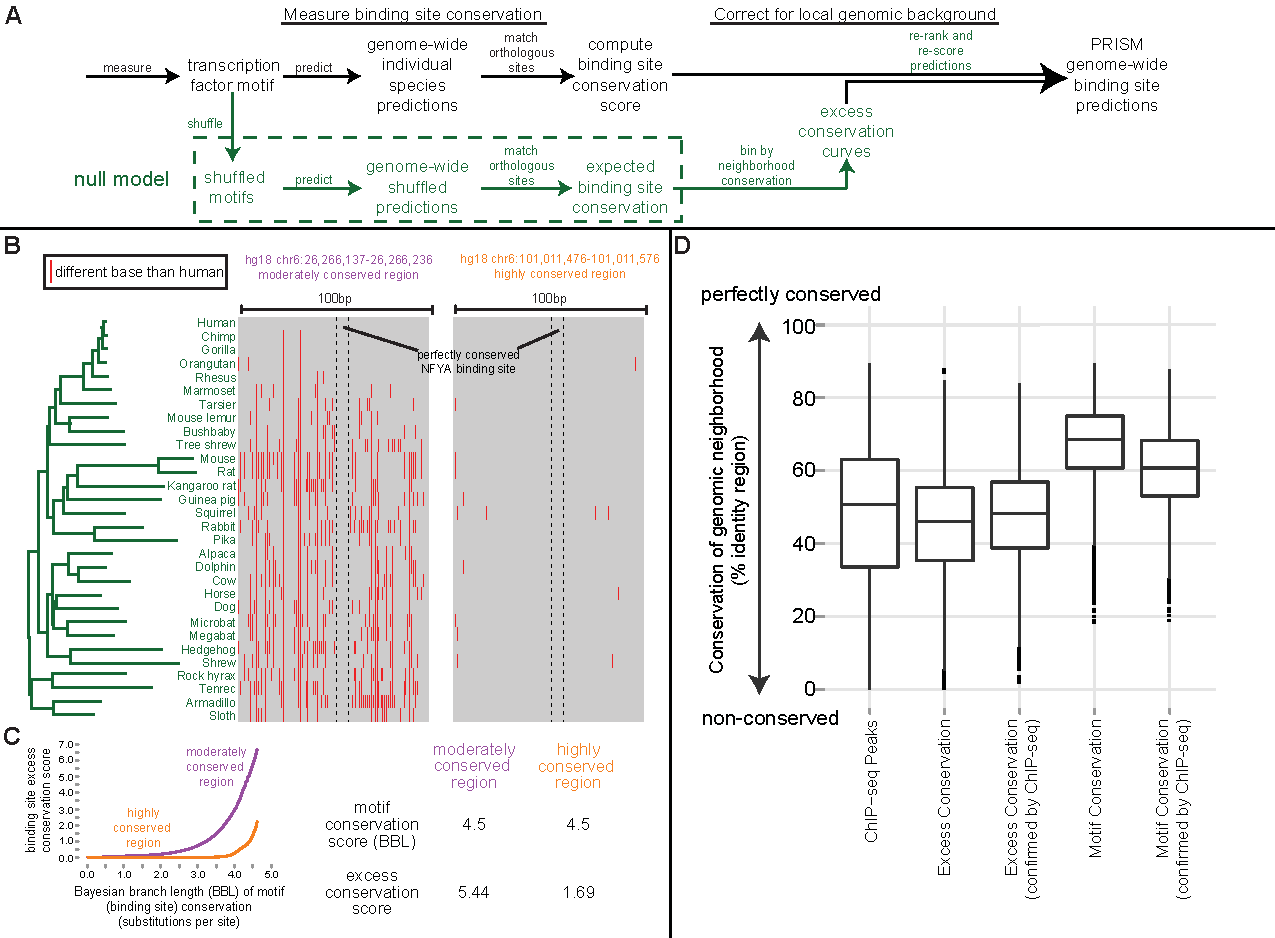
\epsfig{file=figures/prismFig1.pdf,width=0.99\linewidth,clip=,trim=0 0 0 0} \\
\end{tabular}
\caption[PRISM excess conservation rescoring favors predicted transcription factor binding sites conserved above their local environment]{
{\bf PRISM excess conservation rescoring favors predicted transcription factor binding sites conserved above their local environment.}
{\bf (A)} Excess conservation uses the abundance of conserved binding site predictions for shuffled versions of the input motif, in
similarly conserved 100bp genomic neighborhoods, to rescore conserved binding site predictions (framework in green).
{\bf (B)} The NFYA binding site motif is equally conserved in the two shown loci. Yet it is intuitively appealing to consider the left,
less conserved 100bp neighborhood, more likely to conserve an actual NFYA site.
{\bf (C)} Left: Excess conservation plots made from all 100bp neighborhoods conserved like the two loci in panel B. Y axis is
$-log_{10}$ of the likelihood of a shuffled NFYA motif to achieve the motif conservation score on the X axis
or higher by chance. Right: Because shuffled versions of NFYA more easily achieve high motif conservation scores in loci like the
right locus of panel B, the excess conservation score of this NFYA prediction is lower.
{\bf (D)} Excess conservation rescoring is shown to correct motif conservation-only binding site predictions towards the conservation
profile observed in real ChIP-seq peaks. It also outperforms it in area-under-the-curve analysis of 44 (94\%) of 47 analyzed ChIP-seq sets (see text).
}
\label{fig:prismFig1}
\end{figure}

\subsection{Improving transcription factor binding site prediction using excess conservation}
A long line of previous works~\citep{Xie2009} has defined a methodology for predicting conserved binding sites from a
genome-wide multiple alignment and the position weight matrix, or motif, representation of transcription factor binding specificity. However,
focusing on the motif alone ignores the surrounding sequence in which prediction is done. Mammalian genomes are full of long (100 to 1,000bp),
highly conserved non-coding regions~\citep{Waterston2002, Bejerano2004}. The more conserved a longer genomic stretch is, the more likely it
is to include conserved binding site-like patterns in it by chance (see \figref{fig:prismFig1}B). Accounting for this differential likelihood of false
predictions has been valuable in improving earlier methods~\citep{Kheradpour2007}. 

We have developed an adjustment to the latest conservation metrics that accounts for the conservation level of the predicted binding site's
immediate genomic vicinity (\figref{fig:prismFig1}A-C).  We assign each binding site prediction an ``excess conservation'' score which measures
how unlikely it is for the binding site to be conserved by chance to the observed depth in a particular region of the genome based on
the behavior of shuffled versions of its motif in similarly conserved regions of the genome (see Methods in \ref{sec:prismMethods}).  The method explicitly favors
binding sites that are conserved more strongly than surrounding sequence, which suggests evolutionary constraint aimed at transcription
factor binding site preservation (\figref{fig:prismFig1}C). While motif conservation-only metrics gravitate towards prediction in deeply
conserved regions, the excess conservation adjustment produces predictions with a conservation profile matching closely to that of
actual ChIP-seq binding sites (\figref{fig:prismFig1}D). The excess conservation method also more accurately identifies binding sites,
as measured by area under the curve analysis of overlap with ChIP-seq, for 44 of 47 (94\%) examined transcription
factors (\tabref{tab:prismTableS1}).

\begin{figure}[htbp]
\centering
\begin{tabular}{l}
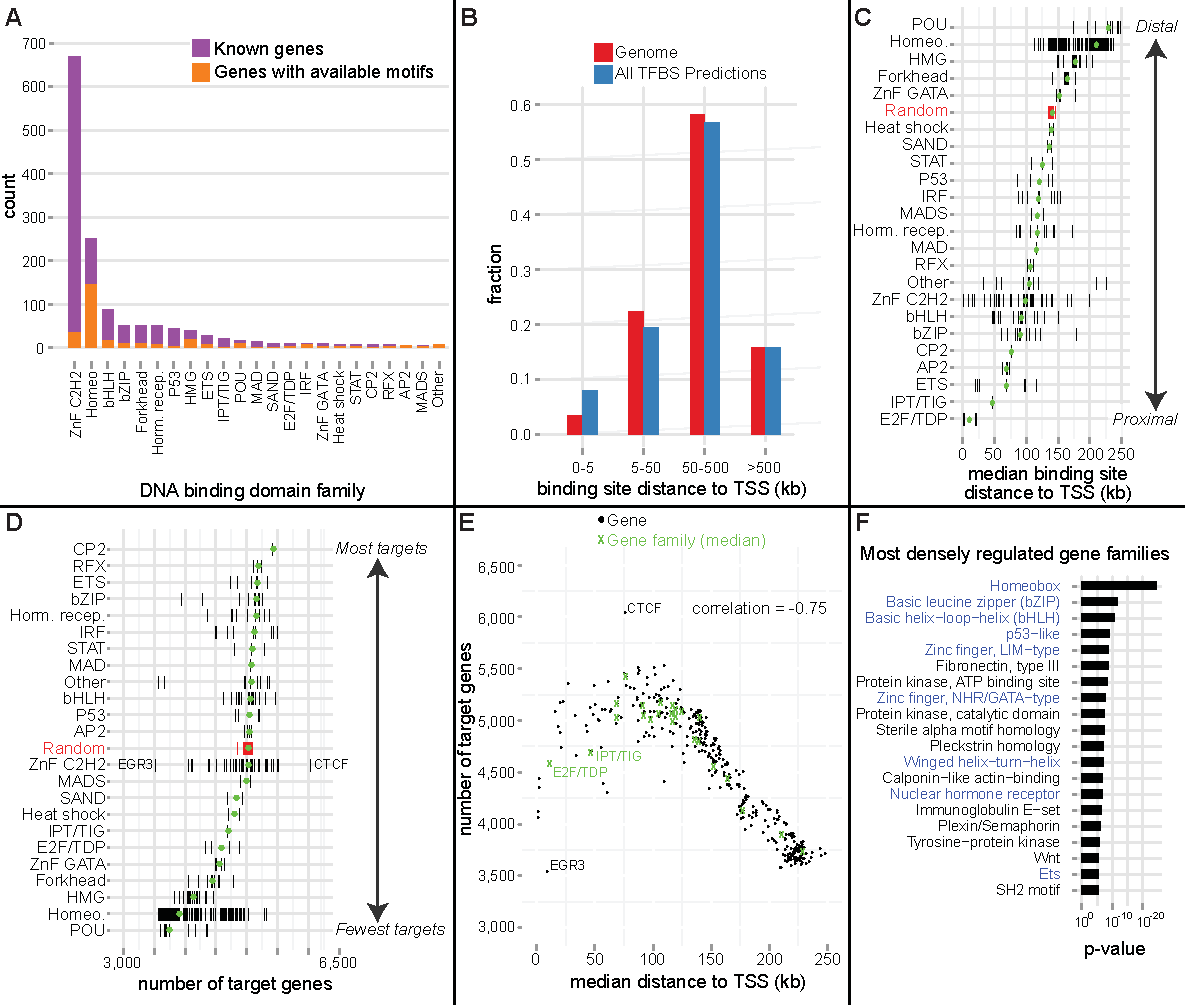
\epsfig{file=figures/prismFig2.pdf,width=0.99\linewidth,clip=,trim=0 0 0 0} \\
\end{tabular}
\caption[Genome-wide excess conservation binding site predictions reveal fundamental properties of mammalian transcription regulation]{
{\bf Genome-wide excess conservation binding site predictions reveal fundamental properties of mammalian transcription regulation.}
{\bf (A)} The curated library of 332 non-redundant high quality transcription factor motifs includes members of all major DNA binding domain families.
{\bf (B)} Distributions of all genomic bases (red) and all conserved binding site predictions (blue) as a function of distance from
transcription start site (TSS). While predictions are 2.3 fold enriched in the proximal promoter, over 90\% of them are distal.
{\bf (C)} Different DNA binding domain families exhibit different binding distance preferences relative to the TSS. Black ticks are median
distances per motif, green dot is the family median, random is the median of 332 uniform shuffles.
{\bf (D)} Number of predicted target genes for the different DNA binding domain families. Black ticks, green dots, and random as in
panel C. POUs and Homeodomains cluster the most around target genes, while CTCF is at the opposite extreme.
{\bf (E)} Distance to TSS and number of target genes have a strong inverse correlation.
{\bf (F)} Transcription factors (blue) are the mostly densely regulated gene families in the human genome, as measured by the fraction of
basepairs in the gene's regulatory domain covered by a binding site prediction.  Shown are all non-redundant significant terms after
Bonferroni correction (see text).
}
\label{fig:prismFig2}
\end{figure}

\subsection{Genome-wide binding site prediction reveals trends in mammalian transcription regulation}
We obtained 389 motifs covering 289 factors from UniPROBE~\citep{Newburger2009}, 133 motifs covering 90 factors from JASPAR~\citep{Bryne2008},
and 294 motifs covering 151 factors from TransFac~\citep{Matys2006}.  After careful semi-automated curation to select only high-quality,
non-redundant motifs (see Methods in \ref{sec:prismMethods}), we obtained 332 motifs, covering at least one member from every major DNA binding domain family (\figref{fig:prismFig2}A).
For each motif, we identified the approximately 5,000 instances genome-wide with the highest excess conservation scores, for a total of
nearly 3.3 million predicted binding sites for the human and mouse genomes across all motifs at a false positive rate of 0.6 (see Methods in \ref{sec:prismMethods}).
While our predictions are encouragingly enriched in the proximal promoter (2.3 fold compared to genome-wide expectation), over 90\% of
binding site predictions lies outside of proximal promoters (\figref{fig:prismFig2}B).

The predictions reveal interesting trends in the propensity of certain DNA binding domain families to target genes more proximally
or distally than others (\figref{fig:prismFig2}C). We associate binding sites to target genes using default GREAT gene regulatory
domains (basal domain: 5kb upstream + 1kb downstream, distal domain: up to 1Mb in each direction to the nearest basal domain), which we
previously have shown is ideal for analysis of distal binding sites from ChIP-seq~\citep{McLean2010}.  For the most proximal family,
the E2F/TDF genes, over 47\% of binding site to target gene associations are within 5kb of the transcription start site (TSS).
Many fewer associations are within 5kb for the most distal families: HMG (4.2\%), Homeodomain (3.6\%), and POU (3.2\%).  In fact, over 93\%
of the predictions for the HMG, Homeodomain, and POU families are more than 100kb from the TSS of the associated target gene.

Interestingly, the transcription factor families with the most distal predictions have the fewest downstream targets, showing a tendency
to cluster around a relatively small number of target genes (\figref{fig:prismFig2}D).  In fact, a clear inverse relationship between
distance to TSS and number of predicted target genes holds across the full set of motifs, with a Pearson correlation of -0.75 (\figref{fig:prismFig2}E).
No family has a markedly wider set of target genes than random expectation, but the C2H2 zinc-finger CTCF motif is a clear
outlier (\figref{fig:prismFig2}D-E), reflecting its special role in genome structure organization~\citep{Phillips2009}.

To examine which genes and gene families are most densely regulated, we calculated the fraction of basepairs in a gene's regulatory domain
that are covered by a binding site prediction. Not surprisingly, HOX genes are among the most densely regulated genes (\tabref{tab:prismTableS3}).
When we grouped all target genes into families using Interpro domain composition and performed a Wilcoxon rank-sum test, numerous
transcription factor families rose to the top, suggesting that the regulators themselves have the most upstream regulation
(\figref{fig:prismFig2}F; \tabref{tab:prismTableS4}).

\begin{table}[htbp]
\begin{center}
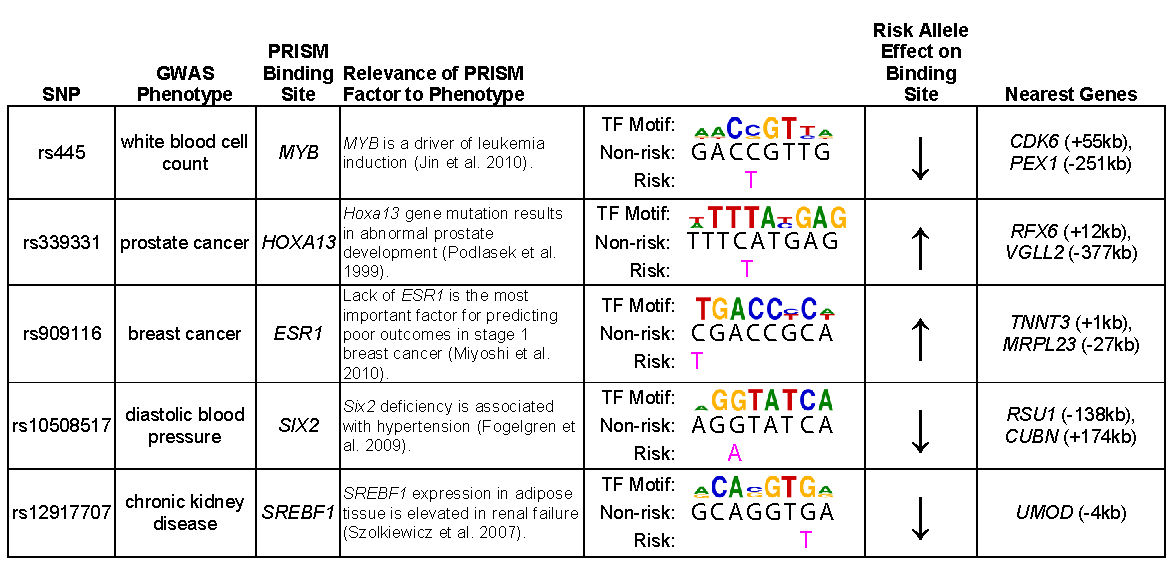
\includegraphics[width=0.99\linewidth]{figures/prismTable1.pdf}
\caption[Biologically appealing PRISM predicted binding sites affected by GWAS risk alleles]{
{\bf Biologically appealing PRISM predicted binding sites affected by GWAS risk alleles.}
PRISM identifies potentially causative binding sites affected by phenotype-associated genome-wide association single
nucleotide polymorphisms.  For the shown cases, the risk allele either weakens (down arrow) or strengthens (up arrow) a
binding site prediction for a transcription factor known to be relevant to the associated disease.
}
\label{tab:prismTable1}
\end{center}
\end{table}

\subsection{Excess conservation binding site predictions overlapping GWAS SNPs}
The NHGRI maintains a catalog of the most significant simple nucleotide polymorphisms (SNPs) associated with a growing number of
diseases and traits, discovered using genome-wide association studies (GWAS)~\citep{Hindorff2009}.  Our excess conservation binding
site predictions overlap 15 of these phenotype-associated SNPs (\tabref{tab:prismTableS5}), a significant overlap (1.86 fold enriched
compared to dbSNP overlap, p-value $< 0.018$, Fisher's exact test, see Methods in \ref{sec:prismMethods}).  For at least five of these SNPs,
the transcription factor that we predict to bind has itself been associated with the phenotype in question (\tabref{tab:prismTable1}).
For example, rs445 is associated (p $< 10^{-7}$) with white blood cell count~\citep{Kamatani2010}.  The risk
allele weakens a predicted binding site for MYB, a key player in the onset of leukemia, a cancer characterized by an abnormal increase
in white blood cells~\citep{Jin2010}.  In other cases, such as rs339331, associated (p $< 10^{-11}$) with prostate
cancer~\citep{Takata2010}, the risk allele strengthens a potential binding site for HOXA13, a key gene for prostate gland
development~\citep{Podlasek1999}.

\begin{table}[htbp]
\begin{center}
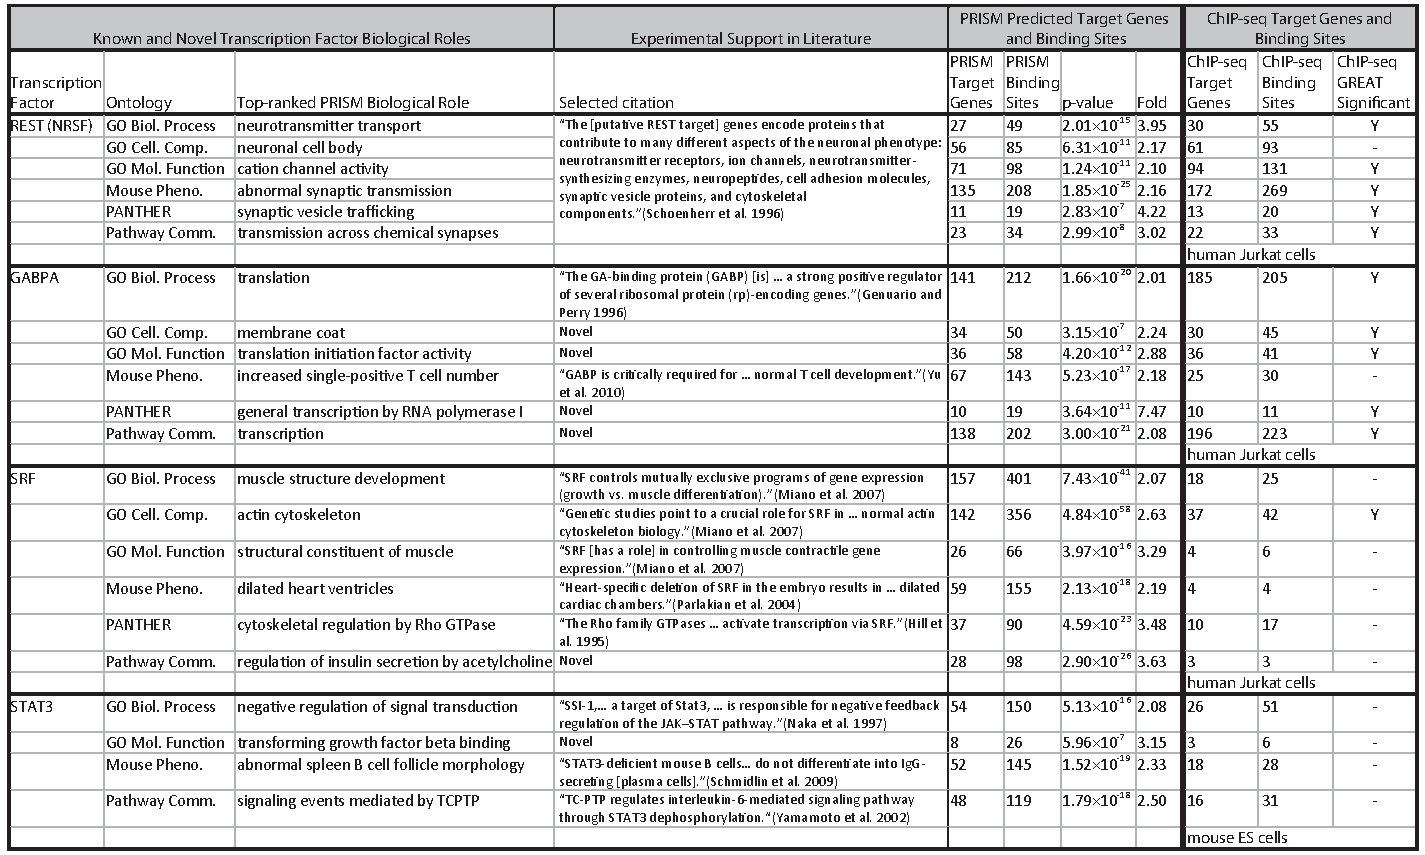
\includegraphics[width=0.99\linewidth]{figures/prismTable2.pdf}
\caption[A comparison of GREAT transcription factor function predictions from PRISM binding site predictions
vs. ChIP-seq peaks for four different factors]{
{\bf A comparison of GREAT transcription factor function predictions from PRISM binding site predictions vs.
ChIP-seq peaks for four different factors.} Columns 2-8: The top PRISM function prediction per ontology for the four
factors highlighted in~\citep{McLean2010}, along with supportive quotes from the literature and PRISM enrichment statistics.
Columns 9-11: A comparison to observed peaks and GREAT enrichments from ChIP-seq in human Jurkat cells or mouse embryonic stem
cells. PRISM independently discovers literature supported functional enrichments observed in ChIP-seq (for \textit{REST} and \textit{GABPA}). By
accessing conserved binding site predictions directly from the genome, PRISM discovers literature supported functions that are
not observed in context specific ChIP-seq experiments (for \textit{SRF} and \textit{STAT3}).
}
\label{tab:prismTable2}
\end{center}
\end{table}

\subsection{Predicting transcription factor functions from binding sites predictions}
We have previously shown that the Genomic Regions Enrichment of Annotations Tool (GREAT)  outperforms gene list-based or microarray-based
tools at revealing biologically meaningful enrichments in ChIP-seq data sets~\citep{McLean2010}.  Our extensive comparisons featured
four transcription factors --  \textit{REST} (\textit{NRSF}), \textit{GABPA}, \textit{SRF}, and \textit{Stat3} -- in both human and mouse contexts, for which GREAT leverages distal
binding sites to reveal accurate and specific function predictions~\citep{McLean2010}.  To compare our transcription factor and
binding site predictions from motif and genome sequence alone to those obtained via antibody ChIP-seq in a particular cellular context,
we predicted binding sites from high quality motifs for the same four factors and analyzed the predictions with GREAT (\tabref{tab:prismTable2}).
 
GREAT analysis of \textit{REST} and \textit{GABPA} binding site predictions substantially agrees with analysis of ChIP-seq peaks for these factors, with
ChIP-seq peaks overlapping 31\% to 71\% of implicated binding site predictions when the enrichments agree
(\tabref{tab:prismTable2}, \tabref{tab:prismTableS6}, \tabref{tab:prismTableS7}).  GREAT analysis of \textit{SRF} ChIP-seq data from human
Jurkat cells generates enrichments that reflect the known role of \textit{SRF} as the master regulator of actin (42 peaks,
p $< 10^{-8}$)~\citep{McLean2010} (\tabref{tab:prismTableS8}).  Using our binding site predictions for \textit{SRF},
we see this same result (p $< 10^{-57}$) from a broad set of 356 binding sites for 142 target genes
(false discovery rate=38\%), the majority of which are not identified in this particular ChIP-seq set (\tabref{tab:prismTable2}).
In addition, 155 of our binding site predictions for \textit{SRF} are strongly associated with genes that cause a dilated heart phenotype when
knocked out (p $< 10^{-17}$; binding site FDR=46\%).  \textit{SRF} is well known for its role in heart development,
and a conditional knockout of \textit{Srf} itself in the developing mouse heart leads to a dilated heart phenotype~\citep{Parlakian2004}.
This experimentally supported result is not found when analyzing the \textit{SRF} ChIP-seq data, which was generated using Jurkat cells,
a T-cell derived cell line unlikely to reflect the biology of the developing heart.

The enrichments for \textit{STAT3} differ markedly between the ChIP-seq and binding site prediction sets.  The top enrichments for the
\textit{Stat3} ChIP-seq data set reflect the context of the experiment, mouse embryonic stem cells (mESC; see \tabref{tab:prismTableS9}).
In contrast, GREAT analysis of genome-wide conserved binding site predictions for \textit{STAT3} highlights its well-known role in
signaling (p $< 10^{-15}$; 150 predicted binding sites; binding site FDR=48\%) and the immune system
(p $< 10^{-18}$; 145 sites; binding site FDR=43\%), two functions with no overlapping peaks in the mESC
ChIP-seq data (\tabref{tab:prismTable2}).  Conserved \textit{STAT3} binding sites and ChIP-seq data thus produce distinct yet complementary
enrichments, which are equally supported by experimental literature.

GREAT analysis of our binding site predictions also produces novel, plausible hypotheses.  For example, 98 predicted \textit{SRF} binding sites
show an association with target genes related to the regulation of insulin secretion (p $< 10^{-25}$; binding site FDR=28\%)
(\tabref{tab:prismTable2}).  While, to our knowledge, this association has not yet been experimentally verified, a recent paper shows that
insulin resistance in humans and mice is marked by increased \textit{SRF} activity~\citep{Jin2011}.  Similarly, GREAT analysis implicates \textit{GABPA} in
regulating ``general transcription by RNA polymerase I'' (p $< 10^{-11}$; 19 binding sites at FDR=13\%), an enzyme
that transcribes ribosomal RNA. \textit{GABPA} is known to regulate transcription of ribosomal proteins~\citep{Genuario1996}.  Our predictions
suggest that \textit{GABPA} may function as a regulator of multiple facets of ribosome synthesis.

\begin{figure}[htbp]
\centering
\begin{tabular}{l}
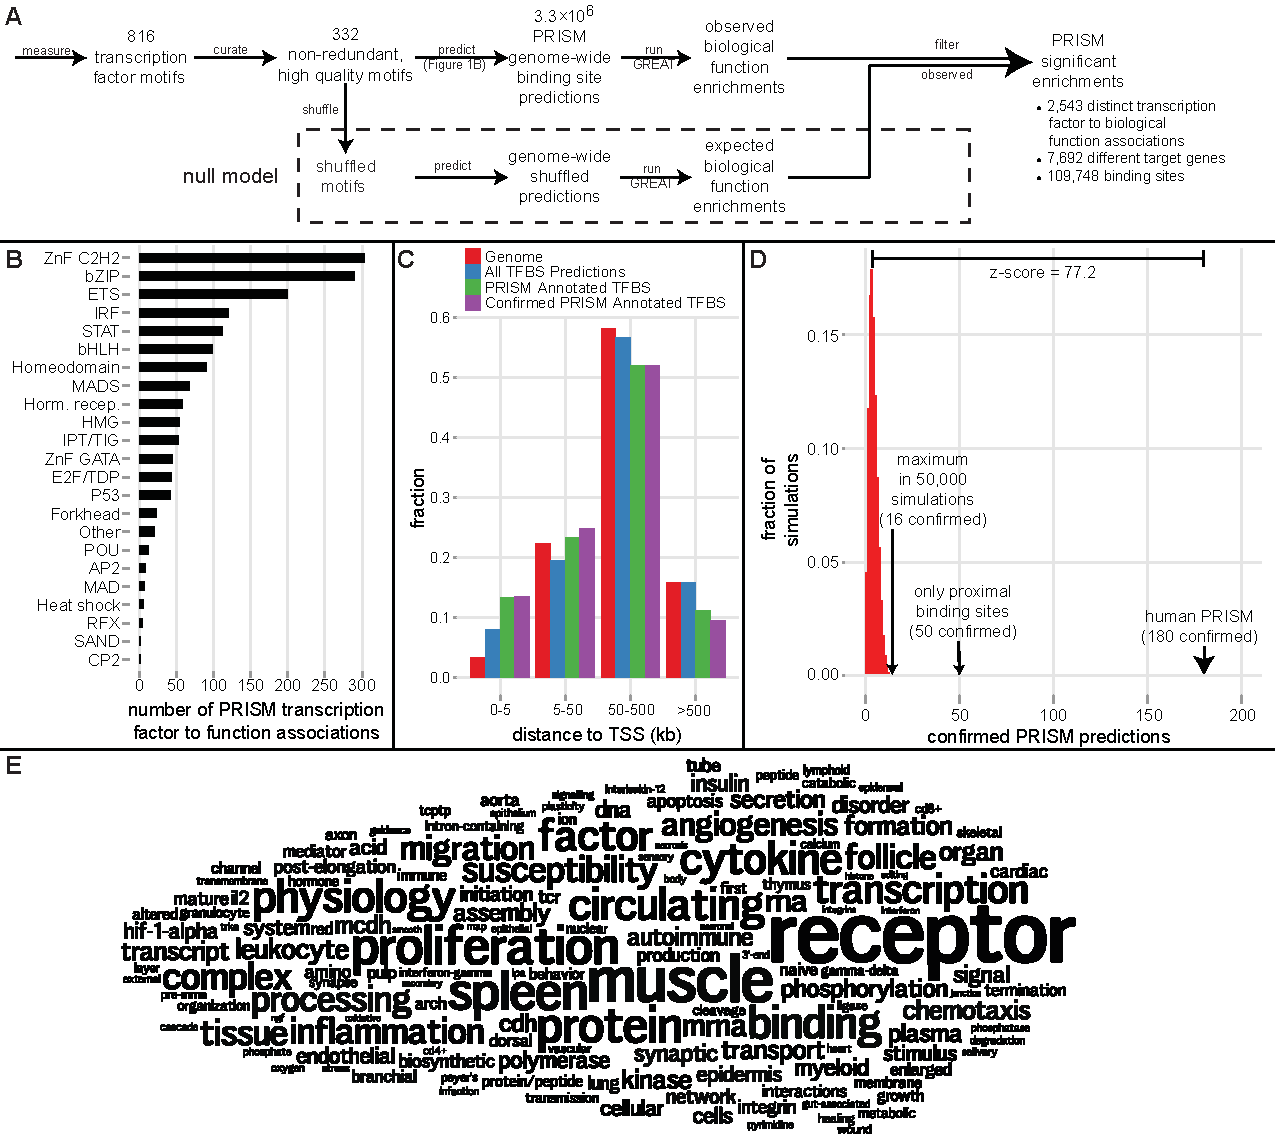
\epsfig{file=figures/prismFig3.pdf,width=0.99\linewidth,clip=,trim=0 0 0 0} \\
\end{tabular}
\caption[PRISM transcription factor and binding site function predictions]{
{\bf PRISM transcription factor and binding site function predictions.}
{\bf (A)} PRISM combines excess conservation binding site prediction (\figref{fig:prismFig1}) with GREAT function prediction from
proximal and distal sites into a novel statistical framework to arrive at thousands of transcription factor (TF) function predictions,
at a false discovery rate of 15\%. Numbers are summed over human and mouse (see text).
{\bf (B)} Distribution of PRISM human TF function prediction across the major DNA binding families.
{\bf (C)} Most of the binding sites that support PRISM predictions -- including high confidence confirmed predictions -- are distal
from putative target genes.
{\bf (D)} PRISM predictions are highly enriched for support by previous literature. The GREAT ontologies tag the transcription
factor itself with the function predicted by PRISM as enriched among its target genes 180 (11\%) times, z-score=77,
p $< 1/50,000$ simulation runs (red); 3.6 fold enriched over using only proximal binding sites.
{\bf (E)} PRISM's 1,658 human TF function predictions cover a variety of biological functions (word size in word cloud proportional to its frequency).
}
\label{fig:prismFig3}
\end{figure}

\subsection{The PRISM framework: predicting biological roles, target genes, and enhancers for hundreds of transcription factors}
Motivated by the biological function predictions obtained for the four different factors, we set to analyze the predicted binding sites
from each of our 332 curated motifs using GREAT~\citep{McLean2010}.  We examined nine GREAT ontologies that provide over 2.4 million
facts about human and mouse gene roles in different biological processes, molecular functions, cellular components, phenotypes,
molecular pathways, and gene families (\tabref{tab:prismTableS10}, see Methods in \ref{sec:prismMethods}). 

While GREAT accounts for multiple hypothesis test correction for multiple ontology terms against a single set of genomic regions,
here we repeatedly apply GREAT to hundreds of sets, one for each motif. To control for multiple hypothesis testing in this framework,
we applied our entire method to the 2,857 shuffled versions of transcription factor motifs used as null models in calculating the
excess conservation score (\figref{fig:prismFig3}A, see Methods in \ref{sec:prismMethods}).  We expect such shuffled motifs, by and large, to lack real functional
signals, though the method is conservative as some shuffles may capture whole or partial binding preferences of uncharacterized
factors and complexes.  For each biological role (annotation term), we used the total fraction of shuffled motifs for which the term
satisfies the GREAT significance thresholds to estimate the expected number of times the term would be falsely called as significant
for a set of 332 motifs.  Any term expected to occur falsely once or more was excluded (see Methods in \ref{sec:prismMethods}).

In summary, we predicted binding sites using the excess conservation method in the human and mouse genomes, analyzed the predictions
with GREAT, and controlled for multiple hypothesis testing using shuffled versions of the same motifs.  We term this combined approach
PRISM for ``Predicting Regulatory Information from Single Motifs'' (\figref{fig:prismFig3}A).  For each transcription factor, PRISM
predicts: 1. biological roles, 2. target genes, 3. binding sites, and implicitly 4. \cis-regulatory elements through which the factor
regulates each target gene in each biological role.

For the human genome, PRISM predicts 1,658 associations between a transcription factor and a biological role
(\figref{fig:prismFig3}B, \figref{fig:prismFigS10}, \figref{fig:prismFigS12}A).  In all, the predictions connect 178 transcription
factors with 5,340 target genes via a wide range of 883 different biological roles (captured as a word cloud in \figref{fig:prismFig3}E)
and 59,135 role-specific binding sites, over 85\% of which are distal ($>$ 5kb from TSS, see \figref{fig:prismFig3}C).
By comparing to the number of enrichments inferred for shuffled motifs, we estimated the function prediction false discovery rate
at 14.8\%.  The approach produces a similar breadth and quality of coverage for the mouse genome -- 1,173 associations connecting 168
factors with 4,993 target genes and 61,437 binding sites through 640 biological roles at an estimated false discovery rate
of 16.1\% (\figref{fig:prismFigS11}, \figref{fig:prismFigS12}B). Combining the human and mouse sets and counting identical orthologous
predictions only once, PRISM predicts 2,543 transcription factor to biological role associations, connecting 217 distinct transcription
factors with 7,692 distinct target genes (see Methods in \ref{sec:prismMethods}).

\subsection{PRISM offers both breadth and depth of biological role predictions}
The same ontologies used by PRISM to infer biological roles of a transcription factor from its predicted binding sites can sometimes
be used to directly confirm a role prediction in an objective, unbiased manner (and thus further support our mostly novel binding
site predictions).  The ontologies provide such support when the transcription factor itself is tagged with the same function that
PRISM identifies as enriched among its downstream target genes.  For example, the PRISM prediction that \textit{GLI2} is involved in
``skeletal system development'' is confirmed by the Gene Ontology, which tags \textit{GLI2} itself with the same term and a supporting
reference~\citep{Mo1997}.  In total, 180 (11\%) of the 1,658 human-based predictions of biological roles for transcription factors
and 145 (12\%) of the 1,173 mouse-based predictions are confirmed this way.
The number of observed confirmations is highly significant (p $< 2\times10^{-5}$), as no more than 16
matches (1\%) were observed in 50,000 simulations that apply a transcription factor's annotations to its shuffled
motifs (\figref{fig:prismFig3}D).

Distal binding sites contribute greatly to the PRISM approach.  With only proximal binding sites (-5kb to +1kb from TSS), PRISM in
human only predicts 50 (3.6 fold less) biological roles which are confirmed by the ontologies (\figref{fig:prismFig3}D), and
only 23 (6.3 fold less) mouse predictions confirmed by the ontologies.

While direct ontology support can confirm function predictions, the lack of such support does not imply an incorrect prediction.
For example, as discussed above, PRISM predicts that \textit{SRF} regulates genes that compose the ``actin cytoskeleton.''  Although \textit{SRF}
is known as the master regulator of the actin cytoskeleton~\citep{Miano2007}, it acts in the nucleus and is not involved in building
the cytoskeleton itself; thus, it is appropriately not annotated with the Gene Ontology Cellular Component term ``actin cytoskeleton.''
Other missing confirmations are due to the incompleteness of annotation.  For example, PRISM predicts 91 \textit{GATA6} binding sites near
23 genes whose mutations lead to abnormal pancreas development (p $< 10^{-12}$; binding site FDR=43\%).  While
\textit{GATA6} currently lacks the same annotation, a very recent study identified \textit{GATA6} as the most common cause of pancreatic agenesis
in humans~\citep{Allen2011}.  Similarly, other unconfirmed PRISM predictions may well represent accurate novel predictions.

PRISM predictions offer not only breadth (as reflected in \figref{fig:prismFig3}E), but can also offer depth and accuracy in terms
of specific function and perturbation predictions. For example, five genes have been previously identified as key master regulators
of muscle differentiation: \textit{MYOD1}, \textit{MYOG}, \textit{MYF5}, \textit{MYF6} (\textit{MRF4}), and \textit{MEF2}~\citep{Pownall2002}. PRISM predicts muscle related roles for
all five (\tabref{tab:prismTableS13}). However, the actual function prediction differs between the factors, reflecting their different
biological roles in muscle formation. PRISM correctly implicates \textit{MYF5} in regulating the myosin complex (p $< 10^{-7}$;
59 sites, binding site FDR=45\%), \textit{MEF2A} in broader regulation of contractile fiber (p $< 10^{-12}$; 128 sites,
binding site FDR=47\%), and \textit{Myod1} in broad regulation of striated muscle tissue development (p $< 10^{-22}$;
236 sites, binding site FDR=50\%). These different functional roles have all been validated experimentally (\tabref{tab:prismTableS13}).
PRISM also offers different perturbation predictions. For example, it predicts that both \textit{MYOG} (p $< 10^{-24}$;
146 sites, binding site FDR=37\%) and \textit{MYF6} (p $< 10^{-10}$; 110 sites, binding site FDR=50\%) disruption results
in general abnormal muscle development.  Both predictions have been validated in mouse (\tabref{tab:prismTableS13}). Furthermore, in
humans, \textit{MYF6} mutations have been associated with Becker muscular dystrophy~\citep{Kerst2000}. For \textit{MEF2A} PRISM predicts disruption
results specifically in abnormal cardiac output (p $< 10^{-5}$; 47 sites, binding site FDR=47\%). Indeed, \textit{Mef2a}
knockout mice suffer from severe heart phenotypes resulting in sudden death associated with heart failure and cardiac arrest~\citep{Naya2002}.

\begin{figure}[htbp]
\centering
\begin{tabular}{l}
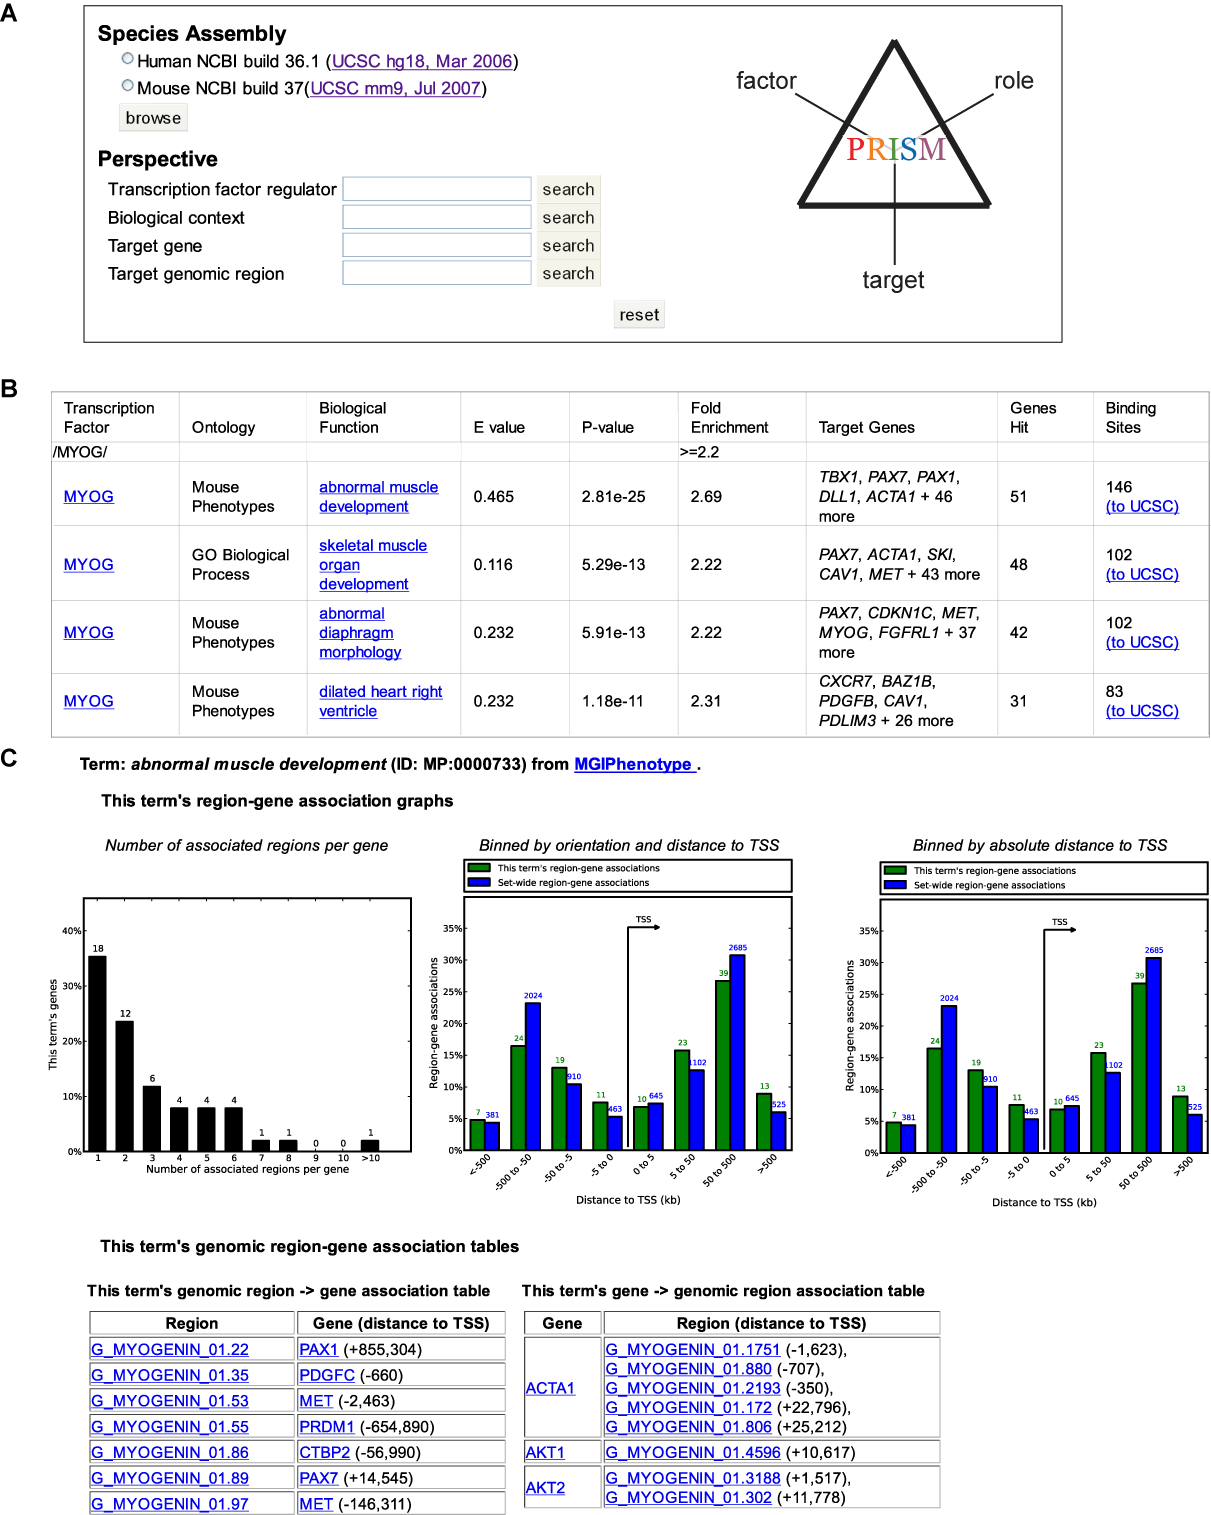
\epsfig{file=figures/prismFig4.png,width=0.8\linewidth,clip=,trim=0 0 0 0} \\
\end{tabular}
\caption[PRISM results are available at PRISM.stanford.edu]{
{\bf PRISM results are available at PRISM.stanford.edu.} Effort has been made to make PRISM current and future predictions
accessible to computational and experimental researchers.
{\bf (A)} The PRISM front page allows browsing the resource, as well as searching for a transcription factor, biological
function, target gene, or target genomic region of interest.
{\bf (B)} The PRISM results page allows advanced filtering on multiple fields and integrates with GREAT and the UCSC genome browser.
{\bf (C)} The term details page for a significant transcription factor role association displays the distribution of supporting binding
site predictions as well as their respective target genes.
}
\label{fig:prismFig4}
\end{figure}

\subsection{The PRISM searchable web portal}
PRISM predictions for the human and mouse genomes are available to the biomedical community at http://PRISM.stanford.edu.  The PRISM portal
offers an interface to explore our predictions from the perspective of transcription factors, biological roles, target genes, or target binding
sites/regions (\figref{fig:prismFig4}).

\section{Methods}
\label{sec:prismMethods}
\subsection{Multiple genome alignments and phylogenetic tree}
All comparative genomic analyses with a human reference utilized the human-anchored Multiz alignment of 44 vertebrates available from
UCSC for the hg18 assembly along with the corresponding phylogenetic tree and branch lengths~\citep{Kent2002}.  Mouse analyses used an
extension of the mm9-based Multiz alignment of 30 vertebrates from UCSC that includes the same 44 species as the human alignment.
Only the eutherian mammals were considered for binding site prediction, and exon and repeat regions were ignored using UCSC annotations.
Similar UCSC hg18-based Multiz alignments of 17 and 28 vertebrates were used for comparison to evaluate trends in multiple alignments
as new species are added.

\subsection{Transcription factor motif library curation}
To obtain a non-redundant set of high quality motifs we combined publicly available motifs from UniPROBE~\citep{Newburger2009},
JASPAR~\citep{Bryne2008}, and TransFac public version 7.0~\citep{Matys2006}. We associated each motif with the gene or genes it
describes.  Because of high redundancy between and within the different resources and low sample sizes for older entries, we
clustered all motifs for a given gene, and used semi-automated curation to identify the highest quality motif/s for each factor.
Among highly similar motifs for the same gene we favored motifs derived from larger sample sizes, and higher information content
respecting general expectations from related family members. This reduced our library from 816 to a high-quality non-redundant
subset of 332 motifs, sampling all major DNA binding domains (\figref{fig:prismFig2}A, \figref{fig:prismFigS5}).

\subsection{Single genome transcription factor binding site prediction}
We predicted binding sites in a single genome or region using position weight matrix models of transcription factor binding
specificity.  Position frequency matrices ($\pi_{i}^{j}$) were converted to position weight
matrices ($\psi_{i}^{j}$) by weighting each column by its information content~\citep{Kel2003}.
\begin{equation}\quad\mbox{Information content of column i:}\quad IC(i) = 2 - \sum_{j \in \{A,C,G,T\} } \pi_{i}^{j} \cdot log_{2} \pi_{i}^{j}\end{equation}
\begin{equation}\quad\mbox{Weight of base j in column i:}\quad \psi_{i}^{j} = IC(i) \cdot \pi_{i}^{j}\end{equation}

Position weight matrix (motif) sequence scores were normalized by dividing by the maximum attainable score.  Sequences with
a score of at least 0.8 (i.e. matching at least 80\% of the possible information content) were considered matches to the motif.

\subsection{Motif shuffling}
For each transcription factor motif, we generated up to ten null model motifs by shuffling its columns.  In shuffling, we preserved
adjacent CpG columns, ensured that the shuffles did not resemble any known transcription factor motif or each other, and maintained
the ``information content profile'' (by only swapping high/low information columns with other columns in the same class defining
0.7 bits as the minimum information of a ``high'' column) (\figref{fig:prismFigS6}).

We defined the similarity of two motifs in a functional manner as the fraction of binding site predictions that overlap.  We
predicted binding sites with the two factors (see above) over a subset of human genomic gene deserts likely depleted for functional
binding events~\citep{Ovcharenko2005}.  For each offset, $i$, at which the two motifs overlap, we counted
the number of overlapping prediction, picked the highest, and normalized:

\begin{equation}
{similarity}(motif_A,motif_B) = \frac{\max_{i} (\mbox{times } motif_A \mbox{ and } motif_B \mbox{ overlap at offset } i)}
{\sqrt{(\mbox{predictions for } motif_A \times \mbox{ predictions for } motif_B)}}
\end{equation}

In generating shuffled motifs, a similarity threshold of 0.2 was used to reject motifs that resemble known transcription
factor motifs or other shuffles of the same motif. This process resulted in 2,857 shuffles for the 332 motifs (\figref{fig:prismFigS7}).

\subsection{Robust binding site prediction across a multiple alignment}
The inclusion of more species in a comparative analysis improves detection of conserved regions~\citep{Margulies2006}, but it also
fragments multiple alignments into smaller blocks (\figref{fig:prismFigS1}).  The fragmentation separates nearby genomic bases in
alignment space, falsely splitting or distancing binding sites across alignment blocks (\figref{fig:prismFigS2}).  To quantify the
effect of alignment fragmentation on prediction sensitivity, we considered the subset of binding site predictions confirmed by overlap
with an ENCODE ChIP-seq peak from \tabref{tab:prismTableS2} (see below).  In a 17-way multiple alignment, 11\% of confirmed binding
site predictions would be lost due to alignment fragmentation without corrective measures, with the loss rate increasing to 16.7\%
in a 44-way alignment, and projected to grow linearly to nearly 30\% of confirmed predictions in a forthcoming alignment of 100 species
(\figref{fig:prismFigS3}).

To overcome this artifact and recover all lost predictions, we padded alignment blocks with 30 basepairs (longer than the longest
analyzed motif) of adjacent sequence from the genomes of all aligned species, collapsed binding site predictions to their single start
coordinate, and placed them on their respective genome (\figref{fig:prismFigS2}A).  To robustly predict conserved binding sites, the
distance between motif matches was defined as the maximum of the distance measured in the reference and non-reference species genomic
coordinates, with the multiple alignment used only to map start positions back to the genome (\figref{fig:prismFigS2}B).  We associated
motif matches at a distance of up to 20 basepairs upstream or downstream, previously shown to be optimal for providing robustness to
biological or artifactual binding site shifting~\citep{Kheradpour2007}.

After associating binding sites in reference and all aligning species, we calculated for every binding site:  1. The number of species
with a matching binding site prediction, 2. The total branch length (BL) of the tree over which the binding site is conserved~\citep{Kheradpour2007},
3. The weighted Bayesian branch length (BBL) which weights phylogenetic distance between species with the binding site match probability
(or quality) in each species. BBL was previously shown to outperform BL for motif conservation score and is extensively discussed
in~\citep{Xie2009}.

\subsection{Efficient conserved binding site prediction}
To predict binding sites, we slide a cursor column-by-column in the multiple alignment, scoring every reference position with all motifs
and retaining all reference binding site predictions in a window.  Given the objective to predict binding sites in the reference genome,
one may avoid scoring sequences in an aligning species if the reference does not contain a corresponding binding site nearby, within the
allowed local misalignment window (\figref{fig:prismFigS4}A).

Implementing this optimization eliminated the need to predict at 90.4\% of aligning positions (\figref{fig:prismFigS4}B), reducing prediction
computation time of the human set from 822 hours to 131 hours (6.3 fold speed-up) on a cluster of Dell PowerEdge 1950 computers with 2.66GHz
Intel Xeon processors and 16GB RAM (\figref{fig:prismFigS4}C).
  
\subsection{Excess conservation score}
The excess conservation framework (\figref{fig:prismFig1}A) rescores every motif binding site prediction according to a null distribution
of scores of shuffled versions of the motif in genomic windows of 100bp of similar conservation level. Formally:
\begin{equation}
\parbox{2cm}{Excess conservation score} = -log_{10}\left( \mbox{Pr} \left\{ \parbox{6cm}{shuffled motif scores in 100bp genomic windows of similar conservation have (shuffled motif score $\geq$ observed real motif score)} \right\} \right)
\end{equation}
To compute it, we partition the reference genome into genomic windows of similar conservation: First, every base in the reference genome is
given a weighted ``\% identity'' score from 0\% (found only in the reference species) to 100\% (same base across the eutherian phylogeny) by
calculating the total branch length over which the reference basepair is matched in the multiple alignment as a fraction of the complete branch
length in the phylogeny.  We then smooth the single position values by averaging over a 100 basepair window centered on it, and group into 1\% bins.

Next, for every motif m we generate a set of shuffles $M_m$ (as above). We predict over the reference genome using all
shuffled motifs and bin the scores for shuffled motifs into frequency histograms according to the genomic conservation bins just described
(\figref{fig:prismFigS8}). We then go back, conceptually, through the reference genome and predict using the motif itself. Every prediction has
a certain motif score, and is done in a genomic 100bp neighborhood of certain conservation. We use the frequency curves for that particular genomic
neighborhood value to derive the empirical p-value of observing the motif score in that conservation neighborhood. The excess conservation score
is $-log_{10}$ of this p-value (see formula above).

Note that the excess conservation framework can be applied to any motif scoring method. Here it is applied to the Bayesian branch
length (BBL) score (above).  As anticipated, when the same motif is equally conserved in two different genomic locations, its excess
conservation score is higher in less conserved genomic windows (\figref{fig:prismFig1}B-C, \figref{fig:prismFigS8}A). In addition, when
two different motifs are equally conserved in equally conserved genomic windows, the motif with higher information content has a higher
excess conservation score, reflecting the higher specificity of its shuffles (\figref{fig:prismFigS8}B).

Binding site predictions in the reference genome were retained, and ranked by excess conservation score, if they were supported by at
least 4 additional species, with a branch length (BL) score of at least 2 substitutions per site and an excess conservation score of
at least 1.3 (i.e. the p-value of the observed motif score in similarly conserved windows = 0.05).

\subsection{Evaluating accuracy of binding site prediction using ChIP-seq data}
We used the UCSC Table Browser to download transcription factors ChIP-seq peaks (binding sites) assayed in human cells by the ENCODE
Consortium~\citep{Encode2011}.  When multiple ChIP-seq experiments or replicates were available for the same factor, we selected the
one with the largest number of peaks, yielding 56 distinct transcription factor sets.  All 47 transcription factors for which we had
a motif in our library were used (\tabref{tab:prismTableS2}).

The accuracy of binding site prediction before and after the excess conservation adjustment is summarized by area under the curve of
precision-recall curves (\tabref{tab:prismTableS1}).  We considered a binding site to overlap a ChIP-seq peak if at least one basepair
overlapped.  The conservation neighborhood for ChIP-seq peaks in \figref{fig:prismFig1}D is measured at the peak center.

\subsection{Identifying binding site overlap with GWAS SNPs}
The NHGRI GWAS catalog of disease-associated SNPs~\citep{Hindorff2009} was obtained from the UCSC genome browser ``gwasCatalog''
track (hg18 assembly).  All PRISM binding site predictions that overlap the SNP by at least one basepair were identified
(\tabref{tab:prismTable1}, \tabref{tab:prismTableS5}).  The association of ESR1 with rs909116 is through a predicted binding site
for the paralogous factor ESRRA (protein similarity BLASTP E-value $< 10^{-45}$).  Statistical enrichment of
overlap of binding site predictions with GWAS SNPs was calculated using a one-tailed Fisher�s exact test:  dbSNP build 130 has
14,985,544 single nucleotide SNPs; the NHGRI GWAS catalog associates 3,776 of these SNPs with a phenotype; PRISM binding site predictions
overlap 32,069 SNPs of which 15 are connected to a phenotype.

\subsection{PRISM \textit{en masse} transcription factor function prediction}
PRISM function predictions were done as follows (\figref{fig:prismFig3}A): For each of our 332 transcription factor motifs, the top
5,000 excess conservation binding site predictions in human and mouse were analyzed using GREAT v1.7~\citep{McLean2010}.  Binding sites
were associated with target genes using the GREAT default ``Basal plus extension'' association rule with default distances of 5kb upstream,
1kb downstream, and up to 1Mb extension, or up to the next gene.  We used the default GREAT filters for significant terms: region-based fold
enrichment = 2, and a region-based and gene-based False Discovery Rate (FDR) Q-value = 0.05, with the additional requirement that at least
5 genes with the term were hit.  Analysis was done over 9 GREAT ontologies -- the 3 Gene Ontology domains~\citep{Ashburner2000}, Mouse
Phenotypes~\citep{Blake2009}, PANTHER Pathway~\citep{Mi2007}, Pathway Commons~\citep{Cerami2006}, BioCyc Pathway~\citep{Caspi2008},
TreeFam~\citep{Ruan2008}, and HGNC Gene Families~\citep{Bruford2008} (\tabref{tab:prismTableS10}).

To provide multiple testing correction for running GREAT 332 times per genome, we used our shuffled motifs. We separately repeated the
entire GREAT analysis with all 2,857 shuffled motifs. For each term we then computed its Expected value (E-value), or number of times it
would appear (by chance) in 332 runs of shuffled motifs:
\begin{equation}
E_{term} = \left(\parbox{6cm}{Fraction of 2,857 shuffled motifs for which the term is significant}\right) \times 332
\end{equation}

When $E_{term} > 1$, the term was removed from the predicted enrichments for real motifs. This resulted in
blacklisting 9\% of the 27,956 human ontology term and 13\% of the 26,656 mouse ontology terms (\figref{fig:prismFigS9}).  To focus on the
top enrichments, we limited to the top 20 terms per ontology for each motif and required an uncorrected region-based GREAT
p-value $= 10^{-5}$, resulting in the human and mouse sets reported in \figref{fig:prismFig3}B, \figref{fig:prismFigS10}, and
\figref{fig:prismFigS11}.

False discovery rates were estimated by comparing the number of factor-role associations for the 332 motifs in the library to the number
of such associations per shuffled motif, after applying multiple testing correction.  For human, the library motifs average 4.99 associations
per motif while the shuffled motifs average 0.74 associations.  For mouse, the library motifs average 3.53 associations per motif and the
shuffled motifs average 0.57.
 
To evaluate PRISM with only proximal binding sites (\figref{fig:prismFig3}D), we analyzed the set of top binding site predictions for each
motif with GREAT v1.7 using only basal regulatory domains (5kb upstream and 1kb downstream of the TSS).  Shuffled motifs were used to calculate
proximal-specific Expected (E) values for terms, which were then filtered as explained above.

To rank target genes, we created a GREAT ontology with each gene as its own term.  Genes were ranked by the region-based binomial p-value, thus
prioritizing genes with an unexpectedly high number of binding sites in the regulatory domain given the size of the assigned domain.

To unify human and mouse predictions, we first manually verified all mappings of motifs to human and mouse transcription factors. We then
mapped orthologous genes and binding sites between species.  Human and mouse orthologous target genes were defined as top BLASTP hits from
the UCSC Table Browser hg18.mmBlastTab table, collapsing transcripts into loci through UCSC gene clusters~\citep{Kent2002}.  Binding site
predictions were considered orthologous if they were identified as nearest matches in the multiple alignment in binding site prediction (see above).

\section{Discussion}
In this study, we developed the PRISM method and resource to predict the functions of transcription factors in the human and mouse
genomes using both proximal and distal binding site predictions.  We provide over 1.6 million conserved binding site predictions per
genome for over 330 different motifs covering all major DNA binding domain families.  The resource also provides a first of a kind
set of over 2,500 transcription factor to biological role associations, each supported by dozens or hundreds of mostly distal novel
binding sites predicted to regulate nearly 7,700 different target genes.  Over 10\% of our role predictions are confirmed by the ontology
annotations of the transcription factor itself, adding further support to the quality of our binding site predictions.  Thus, PRISM
both predicts novel transcription factor roles and extends knowledge of characterized roles by identifying relevant binding sites and
target genes.  These predictions form a valuable resource in the study of mammalian gene regulation.

At the heart of PRISM lies our novel excess conservation score, which refines previous work~\citep{Kheradpour2007, Xie2009} to improve
computational binding site prediction (\figref{fig:prismFig1}).  Conserved binding site prediction does not aspire to replace experimentation.
The binding specificity of transcription factors to DNA is too low, our understanding of the combinatorial rules of transcription
factor synergy and chromatin dynamics is still too poor, and reliance on cross-species conservation hides the majority of experimentally
observed binding sites~\citep{Schmidt2010}.  Nevertheless, those binding sites that are conserved form an \textit{in silico} accessible subset of
likely functional regions, attractively sampling all functions a given transcription factor serves.

When our genome-wide binding site predictions are combined with the millions of facts curated for human and mouse genes and their products,
by placing GREAT in a novel statistical framework (\figref{fig:prismFig3}), we are able to start predicting transcription factor function
\textit{en masse}, while fully leveraging distal binding events. While our individual binding site predictions have moderately high false
discovery rate (60\%), when aggregated into sets with statistically significant shared functions, the false discovery rate of our function
prediction is an appealing 15\%, and the individual binding site FDR improves to 40\%.  One common approach to improve binding site prediction
accuracy is to limit predictions to gene proximal promoters~\citep{Das2006, Down2007, Sinha2008}.  Corroborating virtually all unbiased
ChIP-seq datasets, we show that limiting attention to only the proximal sites ignores the vast majority of genome-wide binding, and in
particular it degrades the number of validated predicted gene functions we make by a marked 3 to 6 fold.

PRISM predictions powerfully complement ChIP-seq experiments. ChIP-seq provides a comprehensive view of binding sites and transcription factor
function in the assayed context. However, the labor and costs associated with generating a high quality antibody, collecting enough cells in the
right context, and sequencing, means ChIP-seq is mostly used to explore in depth the targets of a transcription factor that is already established
or strongly suspected of playing a major role in a given context. PRISM presents an attractive alternative for large scale discovery: by sampling
the full spectrum of transcription factor binding sites and functions directly from the genome, it produces clear testable hypotheses (\tabref{tab:prismTable2}).
Moreover, since a binding site motif can be easily extracted de novo from most ChIP-seq sets~\citep{Chen2008}, every ChIP-seq experiment of
a previously uncharacterized factor, in whatever context, can be enhanced by a complement of conserved binding sites and broad function predictions
using the PRISM approach.

ChIP-seq is only one way of obtaining the binding preference of a transcription factor.  Several other high throughput techniques for
characterizing motifs have been developed recently, including methods based on protein binding microarrays~\citep{Berger2008}, massively parallel
SELEX~\citep{Jolma2010}, microfluidics~\citep{Fordyce2010}, and microwells~\citep{Hallikas2006}.  From early returns on these efforts, we
curated a sample of all major DNA binding domains (\figref{fig:prismFig2}). These technologies will soon provide publicly available motifs for
most of the 1,500 to 2,000 predicted transcription factors in the human genome~\citep{Vaquerizas2009}, all of which can be readily incorporated
into PRISM.

Vertebrate transcription regulation is proving to be a complex affair. Large empty gene deserts are now appreciated to be packed with
conserved non-coding, likely \cis-regulatory, sequence. Transcription factors thought to form narrow cascades, directly binding a handful
of targets, are found to bind thousands of loci in a single context. Adding to this emerging picture, our global analysis suggests that
the transcription factors themselves are among the most densely regulated gene families in the mammalian genome. Here we provide windows
to this complex system by predicting a wide range of functions and targets for a wide range of human and mouse transcription factors and
offering them to the community for further exploration.
